\section{Pianificazione}
Lo sviluppo del progetto è diviso nei seguenti periodi:
\begin{enumerate}
	\item Analisi dei requisiti;
	\item Progettazione architetturale;
	\item Progettazione di dettaglio e codifica;
	\item Validazione e collaudo.
\end{enumerate}
In ogni periodo sono raggruppate le attività da svolgere.
I periodi e le attività delle prime due fasi sono individuati con una maggiore precisione rispetto a quelli successivi. Questo è dovuto alla difficoltà nel prevedere le modalità e i tempi richiesti dalle fasi più remote del progetto.
Nei \glock{diagrammi di Gantt} le barre verdi indicano attività di verifica.

Oltre alle attività riportate di seguito, verranno svolte le attività accessorie consistenti nelle riunioni interne ed esterne e produzione dei relativi verbali. Queste attività coinvolgono tutti i componenti e tutti i ruoli attivi nel periodo. 

\subsection{Analisi dei requisiti (dal 2020-10-22 al 2021-01-17)}

\subsubsection{Ruoli attivi}
\begin{itemize}
	\item Responsabile;
	\item Amministratore;
	\item Analista;
	\item Verificatore.
\end{itemize}

\subsubsection{Periodi e attività}

\paragraph{Primo periodo (dal 2020-10-22 al 2020-11-09)}
Questo periodo comincia con la costituzione del gruppo di progetto. Serve dunque a porre le basi per una comunicazione e collaborazione efficace ed efficiente. Vi si svolgono inoltre attività di ricerca superficiale sui capitolati.

\begin{itemize}
	\item Configurazione degli strumenti collaborativi basilari: comprende la scelta e la configurazione dei mezzi per la comunicazione e il lavoro collaborativo;
	\item Analisi superficiale dei capitolati.
	
\end{itemize}

\paragraph{Secondo Periodo (dal 2020-11-10 al 2020-12-13)}
Gli obiettivi raggiunti in questo periodo sono il consolidamento degli strumenti di collaborazione e l'approfondimento dei capitolati.
\begin{itemize}
	\item Configurazione del \glock{repository}: questa attività comprende la creazione di un repository per la condivisione e il versionamento dei prodotti, ma anche la sua configurazione per la verifica automatica della loro validità;
	\item Raccolta di informazioni dai seminari: stesura di appunti sui seminari, da poter facilmente consultare quando necessario;
	\item Studio dei progetti degli anni passati: questa attività ha il fine di individuare gli errori più comuni e le tecniche da prendere come esempio;
	\item Bozza dello studio di fattibilità;
	\item Bozza delle norme di progetto.
\end{itemize}

\paragraph{Terzo Periodo (dal 2020-12-14 al 2020-01-08)}
Questo periodo segue la scelta del capitolato da affrontare. È dedicato alla sua analisi approfondita e alla stesura della documentazione. 
\begin{itemize}
	\item Stesura delle norme di progetto;
	\item Stesura dello studio di fattibilità;
	\item Stesura del piano di progetto;
	\item Analisi dei requisiti e stesura dell'omonimo documento;
	\item Stesura del piano di qualifica;
	\item Stesura del glossario;
	\item Stesura della lettera di presentazione;
	\item Aggiornamento consuntivo;
	\item Verifica della documentazione.
\end{itemize}

\paragraph{Quarto Periodo (dal 2020-01-09 al 2020-01-17)}
È l'ultimo periodo di analisi dei requisiti. Si concentra quindi sulla preparazione dell'esposizione dei prodotti dei tre periodi precedenti.
\begin{itemize}
	\item Preparazione dell'esposizione;
	\item Verifica dell'esposizione.
\end{itemize}


\begin{landscape}
	\begin{figure}[H]
		\centering
		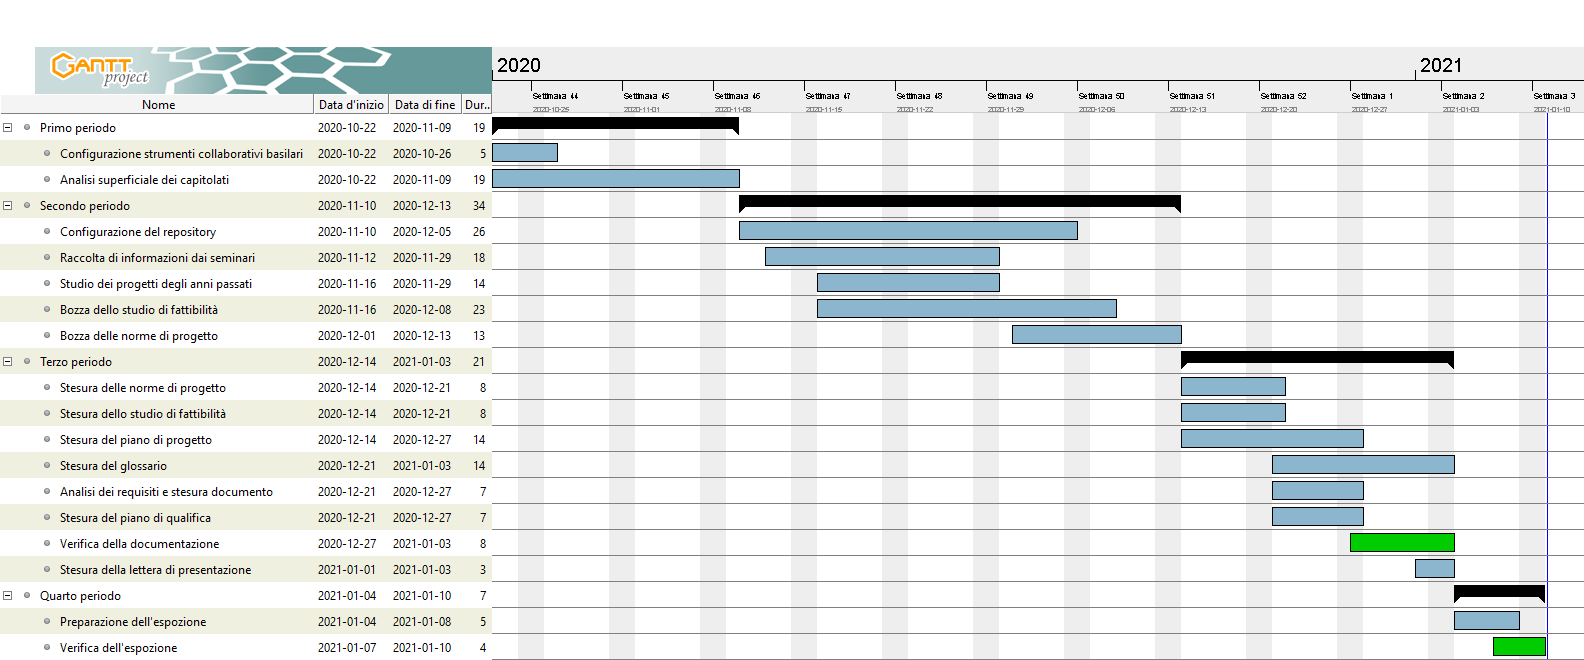
\includegraphics[width=\linewidth]{res/images/ganttFase1.png}
		\caption*{\textbf{Figura 1}{: Grafico di Gantt del periodo di analisi dei requisiti}}
		\label{fig:Gantt Analisi dei requisiti}
	\end{figure}
\end{landscape}

\subsection{Progettazione architetturale (dal 2021-01-18 al 2021-03-07)}

\subsubsection{Ruoli attivi}
\begin{itemize}
	\item Responsabile;
	\item Amministratore;
	\item Analista;
	\item Progettista;
	\item Verificatore.
\end{itemize}

\subsubsection{Periodi e attività}

\paragraph{Primo Periodo (dal 2021-01-18 al 2021-01-20)}
\begin{itemize}
	\item Aggiornamento Norme di progetto;
	\item Aggiornamento Piano di qualifica;
	\item Aggiornamento pianificazione;
	\item Verifica documentazione.
\end{itemize}

\paragraph{Secondo Periodo (dal 2021-01-21 al 2021-02-19)}
\begin{itemize}
	\item Aggiornamento requisiti;
	\item Ricerca: si esegue attività di ricerca sulle architetture più adatte al prodotto da sviluppare e alla soddisfazione dei requisiti richiesti;
	\item Progettazione: si costruisce un modello del prodotto che si vuole ottenere, definendone l'architettura;
	\item Verifica.
\end{itemize}

\paragraph{Terzo Periodo (dal 2021-02-20 al 2021-02-27)}
\begin{itemize}
	\item Progettazione \glock{Proof of concept};
	\item Codifica Proof of concept;
	\item Redazione della  \glock{Technology baseline};
	\item Verifica Proof of concept e Technology baseline.
\end{itemize}

\paragraph{Quarto Periodo (dal 2021-02-28 al 2021-03-07)}
\begin{itemize}
	\item Stesura Lettera di presentazione;
	\item Aggiornamento consuntivo;
	\item Verifica documentazione;
	\item Preparazione presentazione;
	\item Verifica della presentazione.
\end{itemize}

\begin{landscape}
	\begin{figure}[H]
		\centering
		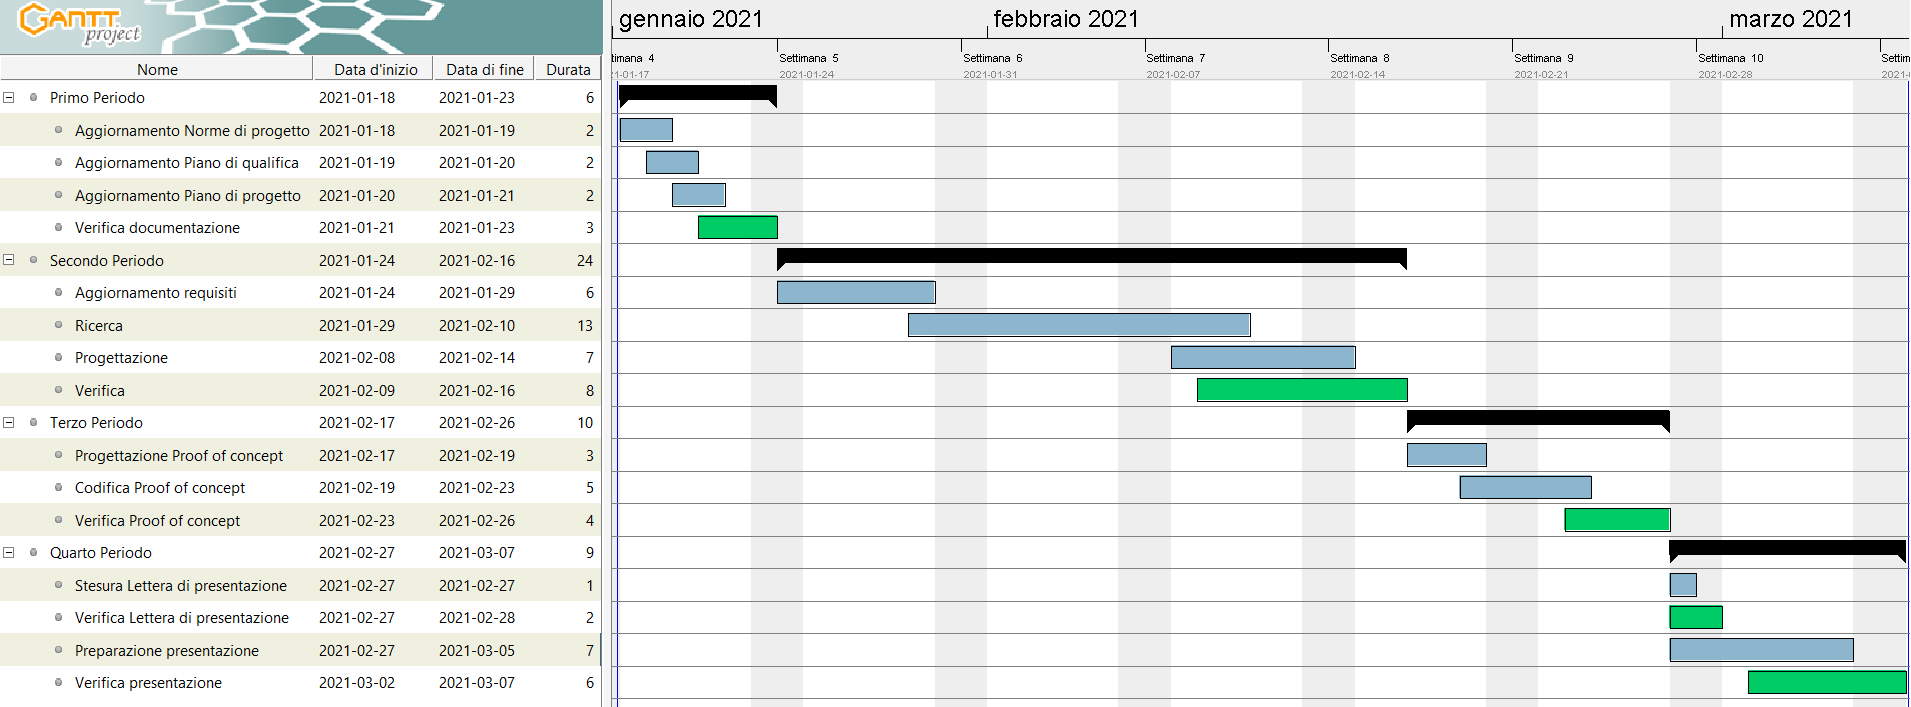
\includegraphics[width=\linewidth]{res/images/ganttFase2.png}
		\caption*{\textbf{Figura 2}{: Grafico di Gantt del periodo di Progettazione architetturale}}
		\label{fig:Gantt Analisi dei requisiti}
	\end{figure}
\end{landscape}